\documentclass[12pt,letterpaper]{article}

% --- Paquetes Requeridos ---
\usepackage[utf8]{inputenc}
\usepackage[spanish,es-tabla]{babel}
\usepackage[margin=2.5cm]{geometry}
\usepackage{graphicx}
\usepackage{float}
\usepackage{titlesec}
\usepackage{setspace}
\usepackage{hyperref}
\usepackage{booktabs}
\usepackage{caption}
\usepackage{enumitem}
\usepackage{listings}
\usepackage{xcolor}

% --- Configuración de Párrafo ---
\onehalfspacing
\setlength{\parindent}{0pt}
\setlength{\parskip}{1em}

% --- Rutas de búsqueda de imágenes ---
% Permite compilar tanto desde Documentos/Entregables/ como con todas las
% imágenes en una sola carpeta plana.
\graphicspath{{./}{../Evidencia/}{Evidencia/}{imagenes/}{../DocumentoFinal/imagenes/}}

% --- Configuración de listings ---
\lstset{
    basicstyle=\ttfamily\footnotesize,
    breaklines=true,
    frame=single,
    captionpos=b,
    showstringspaces=false
}

% --- Inicio del Documento ---
\begin{document}

% --- PORTADA ---
\begin{titlepage}
    \centering

    {\Large \textbf{UNIVERSIDAD SANTO TOMÁS}} \\[1cm]

    {\Large \textbf{Sistema colaborativo de robots móviles para asistencia de orientación en entornos interiores con múltiples pisos}} \\[2cm]

    {\large \textbf{Realizado por:}} \\
    {\large Santiago Hernández Ávila} \\
    {\large Jonny Alejandro Mejía León} \\[1cm]

    \begin{figure}[H]
        \centering
        % Logotipo de la Universidad y la Facultad (en Documentos/, o junto al .tex); si no está, el de la
        % Universidad del documento final.
        \IfFileExists{../Logos Uni.png}{
\includegraphics[width=0.6\textwidth]{../Logos Uni.png}}{%
          \IfFileExists{Logos Uni.png}{\includegraphics[width=0.6\textwidth]{Logos Uni.png}}{%
            \includegraphics[width=0.35\textwidth]{logo_usta.png}}}
        \label{Logo Universidad Santo Tomas y facultad de ingenieria electronica}
    \end{figure}

    \vfill

    {\large \textbf{Informe de Avance --- Semana 29}} \\
    {\large Fase 6: análisis y escritura} \\
    {\large Pruebas de la página y la cancelación, y documento final recortado} \\[1.5cm]

    \textbf{Dirigido por:} \\
    Ing. Armando Mateus Rojas, Msc. \\[1.0cm]

    \vfill

    {\large GED (Grupo de Estudio y Desarrollo en Robótica)} \\
    {\large Facultad de Ingeniería Electrónica} \\
    {\large División de Ingenierías} \\
    {\large Bogotá, noviembre de 2026}
\end{titlepage}

% --- CONTENIDO ---

\section{Introducción}

Este informe presenta el avance de la semana 29 del cronograma (26 de octubre al 1 de noviembre de 2026). Cubre también lo hecho después del corte adelantado de la semana 28, cerrado el martes 20 de octubre, porque ahí quedaron las pruebas del 23 de octubre.

En esas pruebas se verificaron, con un teléfono y los dos vehículos, los ajustes de la página y la cancelación de misiones. Las dos misiones de los ajustes se completaron con relevo, y en las seis cancelaciones hechas después de corregir la media vuelta el vehículo volvió a su escalera dentro de la tolerancia. Al sincronizar el video de esas pruebas se midió que la página mostró la llegada hasta 46,0~s después que el coordinador, lo que corrige la explicación que daba la evidencia de esa sesión (sección~\ref{sec:retraso}). El documento final se recortó de 94 a 77 páginas, dentro del rango de 60 a 80 que pide el director, y se revisó con las anotaciones de los autores. Los 36 requisitos de la matriz quedaron verificados.

Quedan pendientes las autoridades académicas del documento y dejar la versión recortada como la vigente.

\section{Objetivos de la semana}

El cronograma fija para esta semana dos actividades, sin criterio de cierre propio: la sustentación, si la fecha se corría a esta ventana, y definir la estructura del documento final e iniciar su redacción.

La sustentación no se realizó. La Universidad fijó las presustentaciones del 2 al 6 de noviembre, la entrega del documento final el 13 de noviembre y las sustentaciones en la primera semana de diciembre. La estructura y la redacción del documento estaban hechas desde la semana 28; esta semana se recortó y se revisó (sección~\ref{sec:documento}).

De lo previsto en el informe anterior, los ajustes de la página se probaron el 23 de octubre y la restricción RNF-03 (operación en condiciones controladas) se cerró el 27 de octubre (sección~\ref{sec:correcciones}).

\section{Pruebas del 23 de octubre con los dos vehículos}

Se corrieron 18 misiones en los pisos 3 y 4 del edificio Catalayud, con un vehículo por piso. El detalle está en \cite{pruebas} y los registros del coordinador, en \texttt{campo\_20261023/}.

\subsection{Ajustes de la página}

En una misión de bajada (Salón 403 $\rightarrow$ Salón 303) y una de subida (Salón 301 $\rightarrow$ Salón 401), el equipo vio en el teléfono el título de la confirmación según el sentido del cambio de piso. Las dos se completaron con relevo, en 69,4~s y 99,3~s.

\subsection{Cancelación y media vuelta}

Tras cada cancelación o tramo fallido, el programa del vehículo rechazaba la media vuelta. Nav2 guarda varios minutos las metas terminadas, y con una cancelada o abortada en la lista el vehículo se declaraba en error. Sin la media vuelta, Nav2 intentaba girar solo en el pasillo y oscilaba: una misión abortó y un regreso a la escalera falló tras tres intentos. Se corrigió el mismo día, para que la media vuelta se rechace solo con una meta en curso, y se copió a los dos vehículos. Las pruebas automáticas pasan: 50 de 50 del programa del vehículo y 19 de 19 del coordinador con vehículos simulados. Antes de la corrección se rechazaron 8 de 15 medias vueltas; después, ninguna de 10.

Después de la corrección se cancelaron seis misiones, una o más en cada etapa, y en las seis el vehículo volvió a su escalera dentro de la tolerancia de 0,5~m (tabla~\ref{tab:cancelaciones}).

\begin{table}[H]
\centering
\small
\caption{Cancelaciones después de corregir la media vuelta.}
\label{tab:cancelaciones}
\begin{tabular}{@{}p{5.2cm}p{4.6cm}p{5.6cm}@{}}
\toprule
\textbf{Misión} & \textbf{Etapa al cancelar} & \textbf{Distancia a su escalera} \\ \midrule
Salón 302 $\rightarrow$ Salón 402 & Primer tramo, yendo a recoger & 0,173~m (segundo intento; el primero, 0,578~m) \\
Salón 303 $\rightarrow$ Ascensor (piso 3) & Primer tramo & 0,337~m \\
Escalera (piso 3) $\rightarrow$ Salón 402 & Transferencia & 0,074~m \\
Escalera (piso 3) $\rightarrow$ Salón 401 & Esperando confirmación & 0,302~m \\
Salón 401 $\rightarrow$ Salón 303 & Segundo tramo & 0,337~m \\
Ascensor (piso 3) $\rightarrow$ Salón 401 & Segundo tramo & 0,328~m \\ \bottomrule
\end{tabular}
\end{table}

\subsection{Retraso de la página frente al coordinador}
\label{sec:retraso}

El equipo notó lenta la confirmación de la llegada. En el coordinador, del último movimiento del vehículo a la marca de misión completada pasaron 2,03~s y 2,27~s, por la espera de 1,5~s antes de verificar. La evidencia de la sesión atribuía la lentitud a esa espera. Las grabaciones de la pantalla del teléfono muestran que la demora estaba en la página (tabla~\ref{tab:retraso}).

\begin{table}[H]
\centering
\small
\caption{Retraso con que la página mostró el final de cada misión.}
\label{tab:retraso}
\begin{tabular}{@{}p{2.1cm}p{5.6cm}p{2.4cm}p{2.4cm}p{2.3cm}@{}}
\toprule
\textbf{Solicitud} & \textbf{Misión} & \textbf{Marca del coordinador} & \textbf{En la página} & \textbf{Retraso} \\ \midrule
17:18:08 & Salón 403 $\rightarrow$ Salón 303, completada & 17:19:16,97 & 17:20:02,98 & 46,00~s \\
17:20:56 & Salón 301 $\rightarrow$ Salón 401, completada & 17:22:35,70 & 17:23:11,36 & 35,66~s \\
17:33:17 & Salón 302 $\rightarrow$ Salón 402, cancelada & 17:36:02,65 & 17:36:13,11 & 10,47~s \\
Desde las 17:54 & Ocho misiones grabadas & & & De $-$0,04 a 2,00~s \\ \bottomrule
\end{tabular}
\end{table}

La causa no se estableció y no se intentó reproducir. Durante el retraso la página indicaba ``conectado'', y las etapas anteriores de esas misiones habían llegado a tiempo. El requisito RF-18 (la interfaz muestra el estado de la misión) no fija un límite de tiempo, así que su estado no cambia. El retraso queda como observación en la evidencia, corregida con la tabla de las once misiones grabadas, y por decisión de los autores no se declara como limitación en el documento final.

\section{Documento final}
\label{sec:documento}

El documento compila en el equipo del proyecto, sin errores ni referencias sin resolver: la versión vigente (\texttt{main.tex}) tiene 94 páginas y la recortada (\texttt{main\_recorte.tex}), 77.

\subsection{Versión recortada}

El director pide entre 60 y 80 páginas. La versión recortada se armó en paralela, para poder compararla, y reduce el marco referencial, el desarrollo, los resultados, las conclusiones y los trabajos futuros.

\subsection{Revisión con las anotaciones de los autores}

La revisión del 27 de octubre dejó una sola palabra para los robots del proyecto, ``agente'', y los edificios con su nombre: Gregorio (pisos 2 y 3) y Catalayud (pisos 3 y 4), con el cambio de edificio explicado. El texto quedó impersonal, con menos remisiones a otras secciones y con fechas y medidas exactas. Se añadieron figuras de los nodos, del planificador, de la instrumentación y del error de llegada en simulación, y el contrato de interfaces pasó a una tabla. Las conclusiones se reescribieron y los trabajos futuros quedaron en cinco líneas.

La bibliografía pasó de 61 a 42 referencias. El anexo A reúne los ocho videos del proyecto, con enlace y código QR, y el anexo B, el repositorio y el sitio. La pregunta problema quedó con su texto oficial, y el documento nombra a un solo director y la línea de Robótica e Inteligencia Computacional.

\subsection{Preliminares}

De la lista de abreviaturas salieron cinco siglas que el documento no usa (GUI, ICONTEC, MRS, NTC y QoS), y AMCL quedó solo en esa lista. Las etiquetas del mapa del piso 4 se rehicieron, porque la palabra ``salón'' salía con un carácter ilegible. Falta completar los nombres de las autoridades académicas, que hay que tomar de la fuente oficial de la Universidad.

\section{Video de las pruebas}

Con 14 clips de cámara y 4 grabaciones de la pantalla del teléfono se editó un video de 8~min 21~s, a tiempo real y sin audio. A la izquierda va la cámara del usuario y a la derecha la pantalla, en el mismo instante (figura~\ref{fig:video}). Muestra las dos misiones de los ajustes de la página y cinco de las seis cancelaciones; la sexta no quedó en cámara. El video no incluye las cancelaciones anteriores a la corrección de la media vuelta. Se publicó en YouTube el 1 de noviembre (\url{https://youtu.be/31oNn04qLoU}) y es el video 8 del anexo A.

\begin{figure}[H]
    \centering
    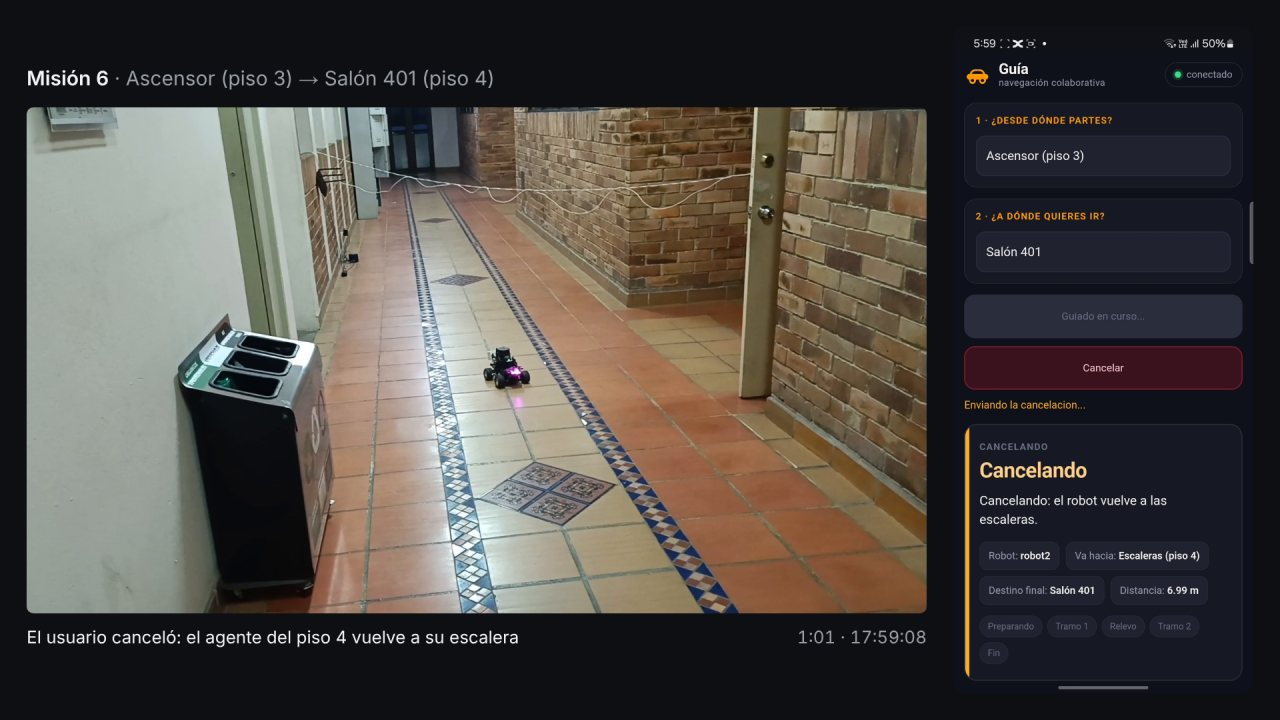
\includegraphics[width=\textwidth]{S29_video_cancelacion_mision6.jpg}
    \caption{Misión 6 del video: el vehículo del piso 4 vuelve a su escalera y el teléfono muestra ``Cancelando''.}
    \label{fig:video}
\end{figure}

Las grabaciones de pantalla no traen hora. Se ubicaron alineando los cambios de título del panel con las marcas del coordinador, y se comprobaron con el reloj del teléfono: el minuto de la barra de estado cambia entre 0,03 y 0,18~s después del segundo 0. La hora del nombre de cada clip de cámara es la de pulsar grabar, y el primer cuadro llega entre 1,48 y 1,75~s después. Por eso cada clip se ubicó con un cambio del panel visible en el teléfono o, si no se veía, con el centro de esa banda. Los cortes de pantalla coinciden con las grabaciones originales con 0,025~s de diferencia o menos. El método y las horas de cada clip están en \cite{video}.

\section{Repositorio y simulación}

El 24 de octubre se ordenó el repositorio: \texttt{ESTADO.md} quedó en una pantalla y su bitácora completa pasó a \texttt{Documentos/historial/}, junto con 25 planes, hojas y guías de sesiones pasadas. Los mundos y modelos de Gazebo pasaron a \texttt{simulacion/}, y el README quedó en 98 líneas.

El 26 de octubre se corrió en el portátil la simulación de dos robots, después de las dos actualizaciones de ROS recibidas desde septiembre: 3 de 3 misiones con relevo, con las llegadas dentro de la tolerancia de 0,25~m \cite{simulacion}. La causa de la falla del 6 de octubre en el otro equipo no se aisló, así que la simulación debe correrse en el equipo que se vaya a usar antes de mostrarla.

\section{Presentación para la presustentación (fuera del cronograma)}

La propuesta de presentación está en \texttt{Documentos/Presentacion/Presustentacion.pptx}, con la plantilla de la presentación del anteproyecto: 39 diapositivas y notas del orador que suman 17~min 20~s. Falta la revisión de los autores.

\section{Correcciones a informes anteriores}
\label{sec:correcciones}

\begin{table}[H]
\centering
\small
\caption{Dato corregido del informe de la semana 28.}
\begin{tabular}{@{}p{2.2cm}p{4.9cm}p{5.6cm}p{2.5cm}@{}}
\toprule
\textbf{Informe} & \textbf{Dato publicado} & \textbf{Dato correcto} & \textbf{Evidencia} \\ \midrule
Semana 28, sección 7 & ``Los videos muestran personas en el pasillo en algunas misiones, y la observación se está registrando misión por misión'' & Los autores confirmaron que en la campaña solo estuvieron en el pasillo ellos dos, que hicieron de usuario, sin personas ajenas que anotar. RNF-03 quedó verificado el 27 de octubre & \texttt{REQUISITOS.md} \\ \bottomrule
\end{tabular}
\end{table}

\section{Aporte a los objetivos específicos}

\begin{table}[H]
\centering
\small
\caption{Trazabilidad de las actividades de la semana.}
\begin{tabular}{@{}p{5.2cm}p{1.6cm}p{8.6cm}@{}}
\toprule
\textbf{Actividad} & \textbf{Objetivo} & \textbf{Aporte} \\ \midrule
Pruebas del 23 de octubre & OE3 & Ajustes de la página y cancelación probados en un teléfono con los dos vehículos \\
Corrección de la media vuelta & OE2 & La maniobra se ejecuta también después de una cancelación \\
Documento final & OE4 & Resultados y conclusiones en la versión recortada y revisada \\
Video de las pruebas & OE3 & Evidencia visual de los ajustes y de cinco cancelaciones, con la pantalla sincronizada \\ \bottomrule
\end{tabular}
\end{table}

\begin{table}[H]
\centering
\small
\caption{Avance por objetivo específico.}
\begin{tabular}{@{}p{1.6cm}p{1.6cm}p{8.6cm}p{2.2cm}@{}}
\toprule
\textbf{Objetivo} & \textbf{Avance} & \textbf{Aporte de la semana} & \textbf{Pendiente} \\ \midrule
OE1 & 100~\% & --- & --- \\
OE2 & 100~\% & Corrección de la media vuelta & --- \\
OE3 & 100~\% & Ajustes y cancelación probados en los vehículos & --- \\
OE4 & 100~\% & Documento recortado y revisado & --- \\ \bottomrule
\end{tabular}
\end{table}

El promedio de los cuatro objetivos sigue en 100~\%, frente al 90,6~\% del calendario (semana 29 de 32). Los 36 requisitos de la matriz están verificados \cite{requisitos}.

\section{Estado del cronograma y trabajo previsto}

\begin{table}[H]
\centering
\small
\caption{Actividades del cronograma para la semana 29 \cite{cronograma}.}
\begin{tabular}{@{}p{6.4cm}p{6.4cm}p{2.6cm}@{}}
\toprule
\textbf{Actividad de la semana} & \textbf{Estado} & \textbf{Evidencia} \\ \midrule
Sustentación, si la fecha se corría a esta ventana & No se realizó: las sustentaciones son en la primera semana de diciembre & --- \\
Definir la estructura del documento final e iniciar la redacción & Hecho desde la semana 28 & Documento final \\ \bottomrule
\end{tabular}
\end{table}

Para las semanas 30 y 31, cuyo criterio de cierre es el borrador completo entregado al director, el equipo prevé:

\begin{enumerate}
    \item Completar las autoridades académicas y dejar la versión recortada como la vigente.
    \item Corregir el nombre de la etapa de cancelación en el registro de misión, actualizar los comentarios con rutas viejas en los dos vehículos y reconstruir la imagen del coordinador.
    \item Incorporar las observaciones de la presustentación.
\end{enumerate}

\section{Conclusiones}

\begin{enumerate}
    \item Los ajustes de la página funcionaron con el teléfono y los dos vehículos, en una misión de bajada y una de subida completadas con relevo.
    \item La cancelación funciona en los vehículos: en las seis cancelaciones hechas después de corregir la media vuelta, el vehículo volvió a su escalera, a entre 0,074 y 0,337~m, dentro de la tolerancia de 0,5~m. Las medias vueltas rechazadas pasaron de 8 de 15 a 0 de 10.
    \item La página mostró el final de tres misiones entre 10,47 y 46,00~s después que el coordinador, todas antes de las 17:54, y de las ocho siguientes con 2,00~s o menos. La causa no se estableció.
    \item La versión recortada del documento tiene 77 páginas, dentro del rango que pide el director, y los 36 requisitos están verificados.
\end{enumerate}

\section{Anexos}

Las cifras de este informe proceden de los registros y documentos de evidencia del repositorio del proyecto, que se listan a continuación. Los videos no se versionan.

\begin{thebibliography}{99}

\bibitem{pruebas}
S. Hernández Ávila y J. A. Mejía León,
``Página y cancelación con los dos vehículos (23 de octubre),''
Repositorio del proyecto, \texttt{Documentos/Evidencia/S28\_campo\_pagina\_cancelacion.md}, noviembre de 2026.

\bibitem{video}
S. Hernández Ávila,
``Video de las pruebas del 23 de octubre, sincronizado con la pantalla del teléfono,''
Repositorio del proyecto, \texttt{Documentos/Evidencia/S29\_video\_pagina\_cancelacion.md}, noviembre de 2026.

\bibitem{simulacion}
S. Hernández Ávila,
``La simulación de dos robots en el portátil, 26 de octubre,''
Repositorio del proyecto, \texttt{Documentos/Evidencia/S29\_simulacion\_relevo\_portatil.md}, octubre de 2026.

\bibitem{cronologia}
S. Hernández Ávila y J. A. Mejía León,
``Cronología del trabajo, semana a semana,''
Repositorio del proyecto, \texttt{Documentos/DocumentoFinal/CRONOLOGIA.md}, noviembre de 2026.

\bibitem{requisitos}
S. Hernández Ávila y J. A. Mejía León,
``Matriz de requisitos,''
Repositorio del proyecto, \texttt{Documentos/REQUISITOS.md}, octubre de 2026.

\bibitem{cronograma}
S. Hernández Ávila y J. A. Mejía León,
``Cronograma de actividades, semanas 17 a 32,''
Repositorio del proyecto, \texttt{Documentos/CRONOGRAMA\_S17\_S32.md}, agosto de 2026.

\end{thebibliography}

\end{document}
